\documentclass{beamer}
\usepackage{tikz}



\title{VennDiagram presentation}
\author{By: Terry Yi, Kelly Ong, Christopher Zaharia, Micheal O'Malley}


\begin{document}
	
	\frame{\titlepage}
	\begin{frame}[t,label=frameA] {Table of Contents}
		\begin{itemize}
			\item{When to Use Venn Diagrams}
			\item{How to Build Venn Diagrams}
			\item{How to label Venn Diagrams}
		\end{itemize}
	\end{frame}
	%Chris Page 1
	\begin{frame}[t,label=frameA]{When to use Venn Diagrams}
		\begin{itemize}
			\item {We can visually represent differences and similarities between two concepts}
			\item {Used to visualize the logical relationships between sets and their elements}
			\item {Showing the interactions between different sets of data, such as the overlap or intersection between two or more sets}
			\item {To visualize the results of a survey or study, showing the distribution of responses across different categories}
			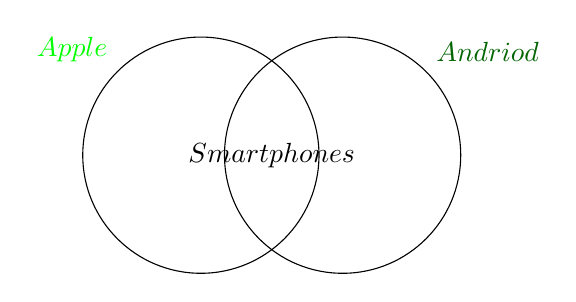
\begin{tikzpicture}
				\node [draw,
				circle,
				minimum size =3cm,
				label={[text={rgb,255:red,0;green,255;blue,0}]135:$Apple$}] (A) at (0,0){};
				
				\node [draw,
				circle,
				minimum size =3cm,
				label={[text={rgb,255:red,0;green,100;blue,0}]45:$Andriod$}] (B) at (1.8,0){};
				
				\node at (0.9,0) {$Smartphones$};	
			\end{tikzpicture}
		\end{itemize}
	\end{frame}
	%Chris Page 2
	\begin{frame}[t,label=frameA]{When to use Venn Diagrams}
		\begin{itemize}
			\item {Demonstration of the different components of a larger system, showing how each component relates to the others}
			\item {The aid in understanding the concepts of union, intersection, and complement in set theory}
			\item {Demonstration of the hierarchy of a system, showing how different levels of the system are related to each other}
			\item {To provide a clear and concise visual summary of complex information, making it easier for the audience to understand and remember}
		\end{itemize}
	\end{frame}

	\begin{frame}[t,label=frameA]{How to Build a Venn Diagram}
		\begin{itemize}
			\item{\textbf{1. Use the "tikz" package}}
			\item{The "tikz" package is a tool used to create graphic elements in LaTeX}
			\item{At the beginning of your document, import the tikz package with " \textbackslash usepackage\{tikz\} "}
%			\begin{figure}[h]
%				\includegraphics[scale=.6]{venn-diagram-code.jpg}
%				\caption{This is the code to create a Venn Diagram in Latex}
%			\end{figure}
		\end{itemize}
	\end{frame}
	
	\begin{frame}[t,label=frameA]{How to Build a Venn Diagram}
		\begin{itemize}
			\item{\textbf{2. How to draw the first circle}}
			\item{INSERT HOW TO DRAW FIRST CIRCLE INSTRUCTIONS}
		\end{itemize}
	\end{frame}
	
	\begin{frame}[t,label=frameA]{How to Build a Venn Diagram}
		\begin{itemize}
			\item{\textbf{3. How to create "Intersection"}}
			\item{INSERT INSTRUCTIONS ON HOW TO CREATE INTERSECTION}
		\end{itemize}
	\end{frame}
	
	\begin{frame}[t,label=frameA] {Complete Venn Diagram}
		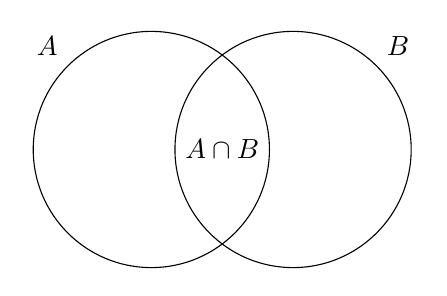
\begin{tikzpicture}
			\node [draw,
			circle,
			minimum size =3cm,
			label={135:$A$}] (A) at (0,0){};
			
			% Set B
			\node [draw,
			circle,
			minimum size =3cm,
			label={45:$B$}] (B) at (1.8,0){};
			
			% Set intersection label
			\node at (0.9,0) {$A\cap B$};
			
		\end{tikzpicture}
	\end{frame}
	
	\begin{frame}[t,label=frameA]{How to label Venn Diagrams}
		\begin{itemize}
			\item {MIKE ADD STUFF HERE}
		\end{itemize}
		
	\end{frame}
	
	
	
	
\end{document}
%Link for basically everything we need :)
%https://latexdraw.com/how-to-draw-venn-diagrams-in-latex/